% ==================================
%             Chapter 4.1
%            Cubic Graphs
%       Created by Michael Tang
%             2025.02.25
% ==================================

\subsection{Cubic Graphs}
\begin{itemize}
    \item \textbf{Cubic Function General Form}
    \begin{equation}
        f(x) = ax^3 + bx^2 + cx + d
    \end{equation}
    Where:
    \begin{itemize}
        \item $a$, $b$, $c$, and $d$ are real numbers.
        \item $a \neq 0$
    \end{itemize}
    \item \textbf{Key Characteristics of Cubic Graphs}
    \begin{itemize}
        \item \textbf{Shape of the Graph}
        \begin{itemize}
            \item The shape of a cubic graph depends on the value of the coefficient $a$.
            \item If $a > 0$, the graph tends to rise on the right and fall on the left (it has an "S" shape).
            \item If $a < 0$, the graph tends to fall on the right and rise on the left (it has an "N" shape).
        \end{itemize}
        \begin{figure}[H]
            \centering
            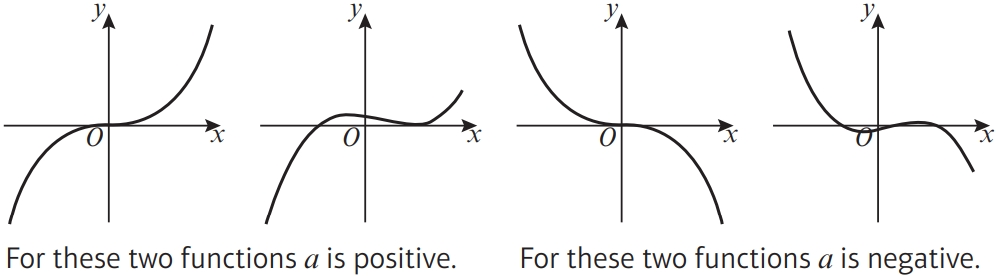
\includegraphics[scale=0.25]{Mathematics/Pure Mathematics/Ch4/Images/Ch4-1-1.png}
        \end{figure}
        \item \textbf{Root of the Cubic Function}
        \begin{itemize}
            \item The points where the graph crosses the x-axis are the roots of the cubic function.
            \item A cubic function can have:
            \begin{itemize}
                \item \textbf{One real root}, where the graph crosses the x-axis once.
                \item \textbf{Two real roots}, where the graph crosses the x-axis at two points.
                \item \textbf{Three real roots}, where the graph crosses the x-axis at three points.
            \end{itemize}
            \item The multiplicity of a root indicates how many times it occurs:
            \begin{itemize}
                \item \textbf{Single root:} The graph crosses the x-axis (i.e., $\left(x - p\right)$).
                \item \textbf{Double root:} The graph touches the x-axis but does not cross it (i.e., $\left(x - p\right)^2$).
                \item \textbf{Triple root:} The graph touches the x-axis and changes direction (i.e., $\left(x - p\right)^3$).
            \end{itemize}
        \end{itemize}
    \end{itemize}
    \item \textbf{General Procedure for Sketching Cubic Graphs}
    \begin{itemize}
        \item[1.] \textbf{Find the roots:} Set $f(x) = 0$ and solve for $x$.
        \item[2.] \textbf{Determine the multiplicity of roots:} This tells you how the graph behaves at each root (cross or
        touch).
        \item[3.] \textbf{Find the y-intercept:} Set $x = 0$ and solve for $y$.
        \item[4.] \textbf{Check the end behavior:} Look at the sign of the leading coefficient $a$ to determine whether the graph
        rises of falls at the end.
        \item[5.] \textbf{Sketch the graph:} Use the roots, y-intercept, and end behavior to sketch the cubic curve.
    \end{itemize}
\end{itemize}